\documentclass[a4paper, 12pt]{article}
\usepackage[utf8]{inputenc}
\usepackage[ngerman]{babel} 
\usepackage{csquotes}

%\author{Frederik Folkers}
%fügt draft hinzu
%\usepackage[pages=all, color=black, position={current page.south}, placement=bottom, scale=1, opacity=1, vshift=5mm]{background}
\usepackage[top=2.5cm, bottom=2cm, right=2.5cm, left=2.5cm]{geometry} % full-width
\usepackage{setspace}

\usepackage{scrlayer-scrpage}
\pagestyle{scrheadings}
\clearpairofpagestyles
\ofoot{\pagemark}

% SQL listings
\usepackage{xcolor,listings}
\usepackage{textcomp}
\usepackage{color}

\definecolor{codegreen}{rgb}{0,0.6,0}
\definecolor{codegray}{rgb}{0.5,0.5,0.5}
\definecolor{codepurple}{HTML}{C42043}
\definecolor{backcolour}{HTML}{F2F2F2}
\definecolor{bookColor}{cmyk}{0,0,0,0.90}  
\color{bookColor}

\lstset{upquote=true}

\lstdefinestyle{SQLstyle}{
    backgroundcolor=\color{backcolour},   
    commentstyle=\color{codegreen},
    keywordstyle=\color{codepurple},
    numberstyle=\numberstyle,
    stringstyle=\color{codepurple},
    basicstyle=\footnotesize\ttfamily,
    breakatwhitespace=false,
    breaklines=true,
    captionpos=b,
    keepspaces=true,
    numbers=left,
    numbersep=10pt,
    showspaces=false,
    showstringspaces=false,
    showtabs=false,
}



\lstset{style=SQLstyle}

\newcommand\numberstyle[1]{%
    \footnotesize
    \color{codegray}%
    \ttfamily
    \ifnum#1<10 0\fi#1 |%
}


% AMS Packages
\usepackage{amsmath}
\usepackage{amsthm}
\usepackage{amssymb}

% Unicode
\usepackage{hyperref}
\hypersetup{
	unicode,
%	colorlinks,
%	breaklinks,
%	urlcolor=cyan, 
%	linkcolor=blue, 
	pdfauthor={Frederik Folkers},
	pdftitle={Entwicklung und Implementation einer Datenbank anhand einer Schulkursbelegung},
	pdfsubject={Datenbanken},
	pdfkeywords={article, template, simple},
	pdfproducer={LaTeX},
	pdfcreator={pdflatex}
}

% BibLaTeX
\usepackage[
backend=biber,
style=alphabetic,
sorting=ynt
]{biblatex}
\addbibresource{Facharbeit.bib}

\usepackage[nottoc,notlot,notlof]{tocbibind} 

% Theorem, Lemma, etc
\theoremstyle{plain}
\newtheorem{theorem}{Theorem}
\newtheorem{corollary}[theorem]{Corollary}
\newtheorem{lemma}[theorem]{Lemma}
\newtheorem{claim}{Claim}[theorem]
\newtheorem{axiom}[theorem]{Axiom}
\newtheorem{conjecture}[theorem]{Conjecture}
\newtheorem{fact}[theorem]{Fact}
\newtheorem{hypothesis}[theorem]{Hypothesis}
\newtheorem{assumption}[theorem]{Assumption}
\newtheorem{proposition}[theorem]{Proposition}
\newtheorem{criterion}[theorem]{Criterion}
\theoremstyle{definition}
\newtheorem{definition}[theorem]{Definition}
\newtheorem{example}[theorem]{Example}
\newtheorem{remark}[theorem]{Remark}
\newtheorem{problem}[theorem]{Problem}
\newtheorem{principle}[theorem]{Principle}

\usepackage{graphicx, wrapfig, color}
\graphicspath{{fig/}}

%\usepackage[linesnumbered,ruled,vlined,commentsnumbered]{algorithm2e} % use algorithm2e for typesetting algorithms
\usepackage{algorithm, algpseudocode} % use algorithm and algorithmicx for typesetting algorithms
\usepackage{mathrsfs} % for \mathscr command

% Author info
\title{\small Facharbeit zum Thema: \\ \Large Entwicklung und Implementation einer Datenbank anhand einer Schulkursbelegung}
%\author{Frederik Folkers}

\date{

}

\begin{document}
	\maketitle
	\thispagestyle{empty}
	
	\begin{center}
	\vspace{3cm}
	\begin{tabular}{ll}
	Schule: & Gymnasium Verl \\
	Schuljahr: & 2021/2022\\
	Kurs: & Grundkurs Informatik\\
	Betreuender Lehrer: & Herr Jansen\\
	\end{tabular} 
	\vfill
	Vorgelegt von:\\
	Frederik Folkers
	\end{center}
	\newpage
	\thispagestyle{empty}
	\tableofcontents	
	\vspace{1cm}
	\begin{center}
	Anhang liegt im USB-Stick bei (UI-Script, Datenbank, Vorbereitungsdateien)
	\end{center}
	\newpage	
	
	\onehalfspace
	\section{Einleitung}
	\label{sec:intro}
	Im heutigen Informationszeitalter ist es wichtig, große und komplexe Datenmengen effizient abzuspeichern und die gewünschten Informationen strukturiert abrufen zu können. Daher habe ich für diese Facharbeit das Thema Datenbanken gewählt. \\
	Zunächst werde ich verschiedene Möglichkeiten zur Sicherung von Daten vorstellen, dann dieses Wissen exemplarisch am Beispiel einer Schulkursbelegung für die Oberstufe darstellen. Bei diesem Projekt folge ich dem einfachen Wasserfallmodell\footnote{vgl. \cite{projModell} S. 328}. Dieses sieht folgendermaßen aus:\\
	\begin{center}
	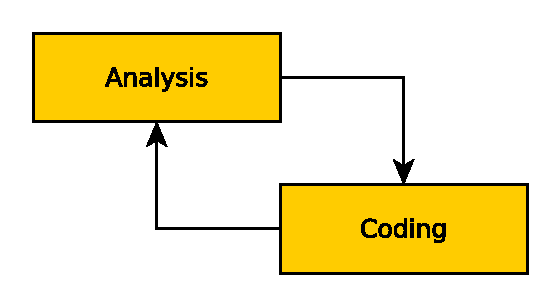
\includegraphics[scale=0.7]{projModell.pdf}
	\end{center}	
	
	Es ist sehr einfach, da es nur aus zwei Schritten besteht: Der Analyse und dem Programmieren. Diese habe ich gewählt, da es ein relativ kleines Projekt ist und die Anzahl der Nutzer höchstwahrscheinlich nicht in den zweistelligen Bereich gehen wird. Allerdings muss noch einen weiterer Schritt hinzugefügt werden:
	\begin{center}
	\includegraphics[scale=0.7]{newprojModell.pdf}
	\end{center}
	
	Die Methodenwahl ist in diesem Fall wichtig, da ich mir am Anfang der Projektes noch nicht sicher war, welche Methoden ich verwenden werde. Dieser Schritt wird die Wahl der Datenbankstruktur, die Wahl des Datenbankmanagementsystems und die Wahl der Programmiersprache beschreiben.
	\section{Problem}
	\label{sec:prob}
	Für diese Facharbeit habe ich mir überlegt, dass ich eine Stundenplanverwaltungssoftware erstellen will. An diesem Beispiel werde ich den Entwicklungsprozess der Datenbankstruktur erklären. Das Problem, welches diese Software lösen könnte, ist die Verwaltung der Individualpläne der Oberstufe. Bei diesen ist, im Gegensatz zu der Unterstufe, das Problem, dass sie, wie der Name schon sagt, individuell sind. Das bedeutet, dass man für jeden einzelnen Schüler der Oberstufe einen eigenen Stundenplan abspeichern muss. Um dies möglichst effizient zu tun, werde ich die Datenbankstruktur auf dieses Problem optimieren. Weitere Funktionen sollten sein, dass man die Raumbelegung, die Schienenzeiten sowie die Namen der Schüler und Lehrer allgemein ändern kann.	
	
	\section{Methodenwahl}
	\label{sec:allgInfo}
		
	
	
	\subsection{Datenbankmodelle}
	\label{sec:dbMod}
	Es gibt verschiedene Datenbankmodelle. Diese unterscheiden sich in ihrer Struktur und Funktionsweise. Die drei Wichtigsten werden in den nächten Abschnitten vorgestellt.
	
	\subsubsection{Hierarchisch}
	\label{sec:hierdb}
	
	\begin{wrapfigure}{r}{6cm}
	\vspace{-28pt}
	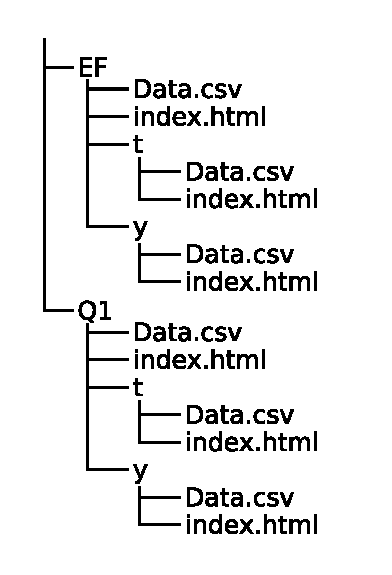
\includegraphics[width=6cm]{vStruk.pdf}
	\vspace{-45pt}
	\caption{Struktur des Vertretungsplans}\label{fig:verTree}
	\end{wrapfigure}
	Ein normales Ordnersystem kann als Datenbankstruktur genutzt werden. Dabei handelt es sich um eine näherungsweise hierarchische Datenbank. Die Informationen werden sehr leicht in Gruppen (durch Unterordner) eingeteilt. Beispiel für die Anwendung einer solchen Struktur ist mein Vertretungsplan. Diesen habe ich als Alternative zu dem normalen Vertretungsplan programmiert. Ich konnte so einige stilistische Verbesserungen einbauen. In der neuen Struktur hat jede Klasse bzw. Stufe ein eigenes Verzeichnis. Dadurch müssen sich die Schüler nicht mehr alle anderen Vertretungen angucken.  Abbildung~\ref{fig:verTree} zeigt die Datenbankstruktur, welche in Form eines Dateisystems angelegt wurde. In jedem Ordner ist eine csv-Datei, in welcher die Daten von der entsprechenden Klasse oder Stufe gespeichert sind. Beiliegend zu jeder csv-Datei ist auch noch eine HTML-Seite. Die beiden Dateien enthalten also grundsätzlich die gleichen Informationen, aber die HTML-Seite ist für Menschen und das csv-Dokument für Maschinen. Ein Vorteil in diesem Fall ist, dass dadurch Daten und Anzeige getrennt sind. So eine Datenbank entspricht aber, wie im ersten Satz angedeutet, nicht in allen Punkten einer hierarchischen Datenbankstruktur. Es gibt zwei große Unterschiede. Wenn in sich in einem Ordnersystem ein leerer Ordner befindet, wird dieser nicht zu einem Blatt (einer Datei). Dies wäre in einer hierarchischen Datenbankstruktur der Fall. Ein weiterer Unterschied ist, dass es keine Beziehungen zwischen den Dateien geben kann.\footnote{vgl. \cite{hierDbWiki}}\\
Dieses Modell hat allerdings auch einige Nachteile, weswegen die Nutzung dieser Struktur bei großen Datenmengen nur eingeschränkt möglich ist. Ein Nachteil ist, dass die Datenbank nur auf einen Anwendung optimiert werden kann\footnote{vgl. \cite{Jarosch2010} S. 117}. Wenn z.B. mein Vertretungsplan nach Tag und nicht nach Klasse sortiert werden soll, müsste die Datenverwaltungssoftware in jeden Ordner reingehen und diesen die entsprechenden Informationen auslesen und abspeichern. Dies ist langsam und leistungsintensiv. Ich habe dieses Problem gelöst, indem ich einen zweiten Ordner für alle eingebaut habe. Das ist allerdings durch die Dopplung nicht sehr effizient. \\
Ein weiteres Problem ist, dass nach einer kleinen Änderung in der Struktur das Programm, ohne Prüfung der Struktur, diese nicht mehr lesen kann\footnote{vgl. \cite{Codd1970} S. 378}. Aktuell ist mein Vertretungsplan nach Klassen sortiert. Wenn ich nun eine Sortierung nach Tagen wollte, müsste das gesamte Verwaltungsprogramm neu geschrieben werden.
	
	\subsubsection{Netzwerk}
	\label{sec:netzdb}
	Die Netzwerkstruktur löst einige Probleme des hierarchischem Datenbankmodells. Bei einer Netzwerkstruktur kann prinzipiell jeder Punkt als Einstiegspunkt verwendet werden. Diese müssen allerdings bei dem Erstellen des Entwurfs festgelegt werden. Das bedeutet, dass man es nicht auf eine bestimmte Sortierung optimieren muss. Beim Erstellen dieses Modells werden die Brücken bzw. Beziehungen schon vordefiniert. Dabei ist es wichtig, dass die Beziehungen in beide Richtungen verwendbar sind. Ein Nachteil dieses Systems ist, dass nur 1:n bzw. n:1 Beziehungen dargestellt werden können\footnote{vgl. \cite{Jarosch2010} S. 119}. 
	
\begin{figure}[h]
\includegraphics[scale=1]{netzwerkmodell.pdf}	
\caption{Netzwerkmodell}\label{fig:netzwerkModell}
\end{figure}

In Abbildung~\ref{fig:netzwerkModell} sind vier Quadrate zu erkennen. Diese stehen für Entitätsmengen. An drei der vier Entitätsmengen sind Ellipsen in denen Einstiegspunkt steht. Ein Einstiegspunkt kennzeichnet im Grunde die Information, die als Ausgangsinformation verwendet werden kann. \\
Wenn nun ermittelt werden soll, in welcher Klasse ein bestimmter Schüler ist, kann der Einstiegspunkt bei Schüler benutzt und von dort aus auf Klasse zugegriffen werden. Dies gilt genauso für Unterrichtsraum und Schule. Wenn erfragt werden soll, welche Klasse einen bestimmten Raum benutzt, oder welche Klassen eine bestimmte Schule hat, so ist das möglich. Wenn aber erfragt werden soll, welcher Klassenraum von einer bestimmten Klasse benutzt wird, ist das genauso wenig möglich, wie herauszufinden welche Schüler in dieser Klasse sind. Der Grund dafür ist, dass Klasse nicht als Einstiegspunkt markiert wurde und somit auch nicht als ein solcher benutzbar ist. Mit anderen Worten: In diesem Beispiel ist es nicht möglich Informationen über Schüler, Unterrichtsräume oder Schulen abzurufen, wenn die einzige gegebene Information die Klasse ist.
		
	\subsubsection{Relational}
	\label{sec:reldb}
	Dieses Datenbankmodell ist das populärste. Die Grundlage dafür bildet das mir vorliegende Artikel „A Relational Model of Data for Large Shared Data Banks” \cite{Codd1970}. Dieses wurde von Edgar F. Codd verfasst und im Juni 1970 veröffentlicht. In diesem Artikel wird eine neue Art der Datenspeicherung vorgestellt. Durch dieses Modell werden einige der Probleme gelöst, welche bei primitiveren Modellen vorhanden waren. Dieser Artikel bildet nebenbei auch noch die Grundlage für die moderne und meistgenutzte Datenbanksprache SQL. \\
Der Artikel beginnt damit, dass der Autor die damaligen Probleme an Datenstrukturen erklärt. Dabei geht er auf das Hierarchische (\ref{sec:hierdb}) und das Netzwerk-Modell (\ref{sec:netzdb}) ein. Daraufhin bringt er ein neues verbessertes Datenbankmodell ins Spiel: Das relationale Datenbankmodell. Dieses Modell basiert darauf, dass die Informationen in zweidimensionalen Tabellen, also Tabellen mit nur einer Spalten und Zeilen Ebene, gespeichert werden. Das hat den Vorteil, dass alle Informationen in einem 2D Array gespeichert werden können. Bei einer dreidimensionalen Tabelle, also wenn mehrere Ebenen existieren, müsste dies durch ein 3D Array dargestellt werden. Das macht die Datenspeicherung unübersichtlich und unnötig kompliziert.\\
Diese Tabellen fassen verschiedenen Entitäts-Typen zusammen wie z.B. „User“, „Bücher“ oder „Verkäufer“. Für jede Eigenschaft der Entitäten wird eine Spalte angelegt. Jetzt kann man immer, wenn man einen neuen Datensatz bzw. Entität in die Tabelle einspeichern will, eine weitere Zeile zu der Tabelle hinzufügen. Jede dieser Tabellen hat einen sogenannten Primary Key. Dieser kann jede Zeile individuell identifizieren. Er kann auch aus mehreren Spalten bestehen. Damit man diese Spalte erkennen kann, ist sie meistens gekennzeichnet. Somit muss Primary Key bei jeder Entität anders sein. Wenn es jetzt Sinn macht einige Informationen in einer anderen Tabelle zu speichern z.B. wenn man ein Bibliotheksverwaltungsprogramm hat, kann man den Inhalt getrennt von dem Regal abspeichern. Für diesen Fall hatte E. F. Codd eine Idee. Man kann eine zweite Tabelle erstellen, in der man alle Informationen zu seinem zweiten Datensatz abspeichert. Um erkennen zu können, welche Zeile zu welcher Zeile in der zweiten Tabelle gehört, fügt man der zweiten Tabelle den Primary Key des ersten hinzu. In der zweiten Tabelle wird dieser dann Foreign Key genannt. Wenn man z.B. nach einem Buch mit einem bestimmten Inhalt sucht, kann man diesen in der Inhaltstabelle suchen und dann in der Regalpositionsliste schauen, wo es steht. Andersherum kann man ein bestimmtes Buch aus der Regalpositionsliste heraussuchen und dann nachschauen, wie der Inhalt ist. Man kann hier einen großen Unterschied zur Netzwerkstruktur erkennen, da man jede Tabelle als Eintrittspunkt nutzen kann. Diese Beziehung wird 1:1 Beziehung genannt, da jede Zeile nur auf eine Zeile verweist. Im Beispiel wird dadurch beschrieben, dass jedes Buch nur einen Inhalt haben kann. Bei dieser Beziehung ist es egal, in welcher Tabelle den Foreign Key steht.\\
Eine 1:n Beziehung ist sehr ähnlich aufgebaut. Bei dieser wird der Primary Key genauso in die andere Tabelle geschrieben. Es ist aber möglich, dass der Primary Key auf mehrere Foreign Keys verweist. In unserem Beispiel würde diese Beziehung genutzt werden, wenn man eine statt einer Regalpositionsliste nur eine Regalliste hätte. In dieser würde dann nur das Regal abgespeichert werden. Damit kann jedes Regal mehrere Bücher haben, jedes Buch aber nur ein Regal. In diesem Fall würde man den Foreign Key in die Bücherliste schreiben.\\
Die letzte Beziehung, mit der ich mich beschäftigen werde, ist eine n:m Beziehung. Diese ist etwas komplizierter, da es nötig wird eine neue Tabelle zu erstellen. Diese Tabelle setzt sich aus den beiden Foreign Keys der Tabelle zusammen, welche beide als Primary Key der neuen Tabelle dienen. Wenn man nun herausfinden will, welche Zeilen der einen Tabelle zur anderen gehören, guckt man einfach den entsprechenden Primary Key in der Beziehungstabelle nach. Dadurch findet man die Primary Keys der entsprechenden Zeilen der zweiten Tabelle und kann diese auslesen. Dieser Vorgang kann auch andersherum benutzt werden. Mit dieser Struktur ist es möglich, große Datenmengen relativ einfach abzuspeichern und diese in Verbindung zu setzten.

	\subsubsection{Entscheidung}
	Ich habe mich für das relationale Datenbankmodell entschieden, da es das modernste und flexibelste ist. Für die Implementierung der Schulkursbelegung ist diese Flexibilität nötig, da ich keine Begrenzung in den Abfragemöglichkeiten haben will. Zudem möchte ich die Programmierung in SQL nutzen. 
	
	\subsection{Datenbankmanagementsysteme}
	\label{sec:dbArten}
	In den 70er Jahren wurde von IBM ein neues Datenbankmanagementsysteme entwickelt, das System R. Um die Daten zu verwalten wurde SQL auf Basis der Erkenntnisse von E. F. Codd entwickelt. SQL steht für \glqq Structured Query Language\grqq{} und wird dazu genutzt, Datenbankstrukturen in relationalen Datenbanken zu erstellen\footnote{vgl. \cite{laube19} S.19}. Zudem können die Daten mit SQL bearbeitet und abgefragt werden\footnote{vgl. \cite{SQLver}}. 
	
	\subsubsection{MySQL}
	\label{sec:MySQL}
	MySQL ist ein Server basiertes Datenbankmanagementsystem. Das bedeutet, es ist möglich mit verschiedenen Benutzern auf dieses System zuzugreifen. Das hat den Vorteil, dass es von mehreren Programmen gleichzeitig genutzt werden kann, diese müssen sich nicht einmal auf dem gleichen Computer befinden. MySQL kann sehr große Mengen an Daten abspeichern, ohne sich dabei zu verlangsamen.
	
	\subsubsection{SQLite}
	\label{sec:SQLite}
	SQLite ist ein einfaches und kleineres Datenbanksystem.  „Lite“ bezieht sich auf die Menge des Speicherplatzes, es wird deutlich weniger benötigt. Um mit der Datenbank zu kommunizieren, wird SQL genutzt. Pro Zeile kann 1 Gigabyte an Daten gespeichert werden und es kann maximal 281 Terabyte an Daten speichern. Ein großer Vorteil dieses Datenbanksystems ist, dass es keinen Server benötigt. Die gesamte Datenbank kann einfach als Datei gespeichert werden\footnote{vgl. \cite{SQLite}}. Aus diesem Grund wird es oft in kleinen Anwendungen benutzt. Am weitesten ist diese Datenbank auf dem Smartphone Markt verbreitet. SQLite schätzt die Anzahl der aktiv benutzten Datenbanken auf über 1 Billionen\footnote{\cite{SQLiteUser}}. Des Weiteren ist SQLite Open Source.
	
	
	\subsubsection{Entscheidung}
	Für dieses Projekt ist meiner Meinung nach SQLite klar die bessere Wahl. Ein Aspekt ist, dass ich dass ich die Datenbank abgeben muss,  deswegen sollte diese auch unabhängig von dem Status irgendeines Servers sein. Allerdings ist es sehr einfach zwischen den Datenbanken zu wechseln, da sie beide SQL benutzen. Dadurch müssen die Befehle nur einmal konstruiert werden und funktionieren dann für beide Datenbanken. Deswegen habe ich beide implementiert.
	
	\subsection{Programmiersprache}
	Bei der Programmiersprache habe ich mir folgende mögliche Kanidaten angesehen.
	\subsubsection{Python}
	\label{sec:py}
	Pyhton ist eine einfache Scriptingsprache, mit der ich schon Erfahrung sammeln konnte\footnote{siehe Vertretungsplan: \ref{sec:hierdb}}.  ist sie gut strukturiert und perfekt für schnelle Programme\footnote{vgl. \cite{Dave13} S.13}.
	
	\subsubsection{PHP}
	\label{sec:php}
	PHP ist eine relativ einfache Programmiersprache zum Programmieren des Backends von Websites. Schon im ersten Jahr wurde eine SQL Funktion eingebaut\footnote{vgl. \cite{phpGesch}}. Dazu hat es mehrere nützliche Funktionen wie 'associative array' bei denen den verschiedenen Objekten statt Nummern Namen zugewiesen werden. Dies ist insbesondere beim Auslesen von Tabellenzeilen nützlich.
	
	\subsubsection{Entscheidung}
	Ich habe mich in diesem Fall für Python entschieden, da es im Gegensatz zu PHP keinen Webserver benötigt, um zu funktionieren. Außerdem wäre es in PHP nötig mehrere html-Seiten zu designen.
	
	\section{Analyse}
	\label{sec:loes}
	Zu der Analyse gehört das Beschreiben eines Programmes. Dies geschieht in diesem Fall durch ein Entity-Relationship-Diagram. Die Syntax eines solchen werde ich im folgendem Kapitel erklären. Danach werde ich mein eigenes Diagramm erklären.
	
	\subsection{Entity-Relationship-Diagramm erstellen}
	\label{sec:ERDers}
	\subsubsection{Syntax}
	\label{sec:ERSyntax}
	Nach der Idee für die Datenbank wird zuerst eine Entity-Relationship-Diagramm erstellt. Dieses wird genutzt um die Datenbank genau zu planen. Bevor wir uns mein Diagramm ansehen könnnen, werde ich zuerst an Abbildung \ref{fig:eBeis} die Syntax erklären.
	\begin{center}
	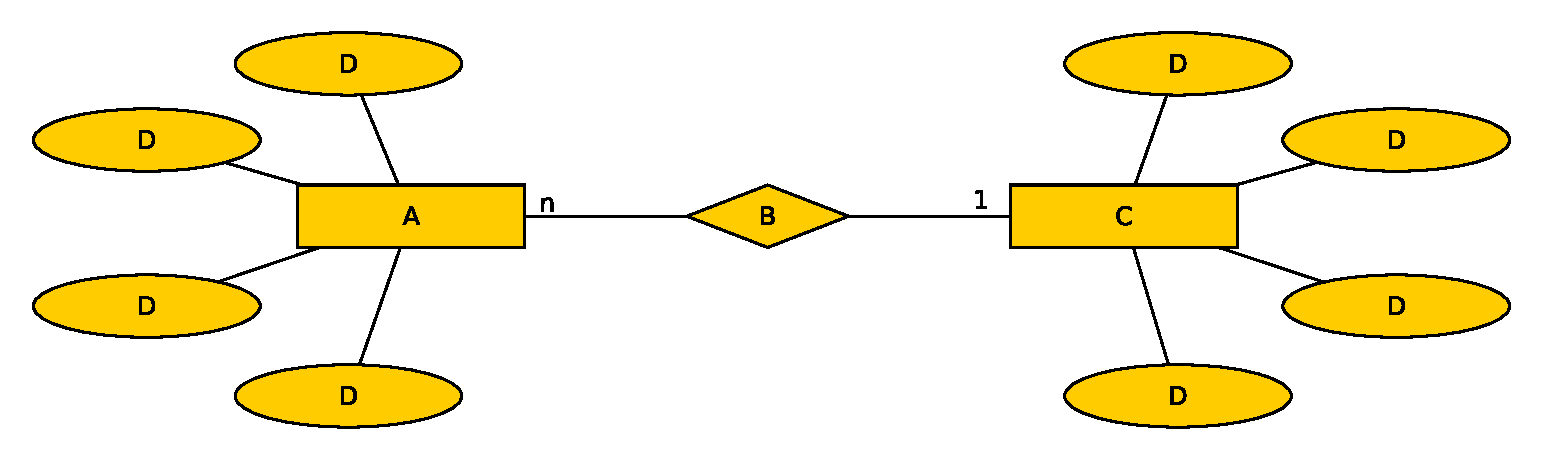
\includegraphics[scale=0.6, ]{EntityBeis.pdf}
	\label{fig:eBeis}
	\end{center}
	
	\paragraph{Attribut (D)} In dieser Grafik werden die Attribute bzw. Spalten durch Ellipsen dargestellt. In einer bildlichen Darstellung durch Tabellen würden Domänen die Spaltenüberschriften repräsentieren. Eine Domäne kann als Primary Key für eine Entitätsmenge gekennzeichnet werden. Dies geschieht, indem man den Spaltennamen unterstreicht\footnote{vgl. \cite{Info2} S. 323}.
	
	\paragraph{Entitätsmenge (A, B)} Die Entitätsmengen werden durch Vierecke dargestellt. Im übertragenen Sinne sind dies Tabellen. Entitätsmengen sind von Attributen umringt. Davon ist normaler Weise mindestens eines ein Primary Key\footnote{vgl. \cite{Info2} S. 323}.
	
	\paragraph{Beziehungsmenge (B)} Eine Raute beschreibt eine Beziehungsmenge. In der Mitte steht die reale Beziehung zwischen den Entitätsmengen z.B. „besitzt“ oder „ist in“. Die Raute ist mit zwei Strichen mit den zugehörigen Entitätsmengen verbunden.  Auf diesen Pfeilen werden die Kardinalitäten notiert. Dabei steht die Menge der Beziehungen einer einzelnen Entität auf der anderen Seite der Raute. In dem abgebildeten Beispiel kann eine Zeile in A nur auf einen Zeile in C verweisen, aber eine Zeile in C kann auf beliebig viele Zeilen in A verweisen\footnote{vgl. \cite{Info2} S. 324}. 
	\subsubsection{ER-Diagramm}
	\label{sec:ERDia}
	\begin{figure}[h]
	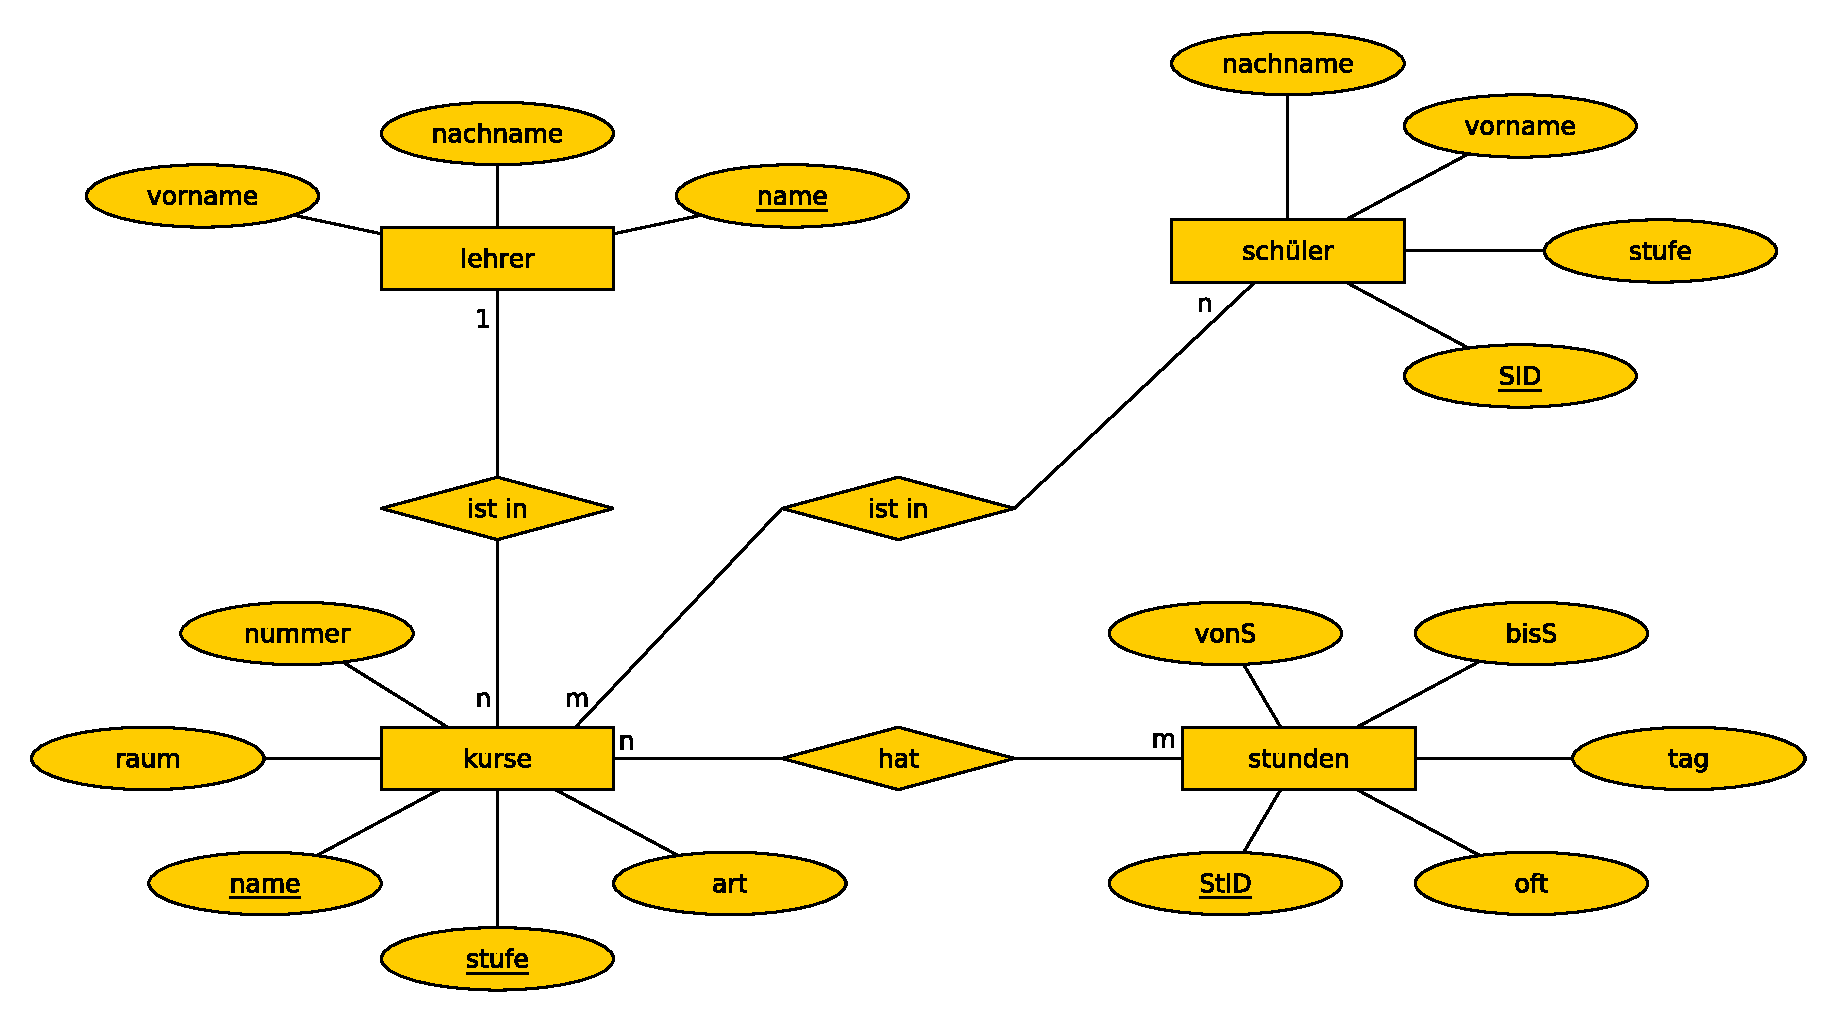
\includegraphics[scale=0.5]{ERStund.pdf}
	\caption{Stundenplan ER-Diagramm}
	\label{fig:ERStund}
	\end{figure}
In Abbildung \ref{fig:ERStund} wird das Stundenplan ER-Diagramm dargestellt. Die folgenden Abschnitte erklären die Einzelheiten.
\paragraph{Schüler}Hier wird für jeden Schüler eine Entität hinzugefügt. Von jedem Schüler wird der Vorname, der Nachname und die Stufe abgespeichert. Des Weiteren wird jedem Schüler eine „SID“(Schüler Identitätsnummer) zugewiesen. Diese dient als Primary Key. Dieser Schritt ermöglicht es mehrere Schüler mit dem gleichen Namen und Nachnamen, welche in derselben Stufe sind, unabhängig voneinander zu verwalten. Der Name „stufe“ ist etwas irreführend, da dieses Attribute die Klasse speichert dabei sind Oberstufe und Unterstufe gleichberechtigt. Also kann hier „8b“ und „EF“ stehen.

%Die Beziehung zwischen Schüler und Kurse ist eine n:m Beziehung, da ein Schüler in mehreren Kursen ist und an den Kursen mehrere Schüler teilnehmen. 
\paragraph{Kurse} In der Entitätsmenge Kurse werden alle besetzbaren Kurse zusammengefasst. Dabei werden die Werte „stufe“, „name“, „fach“ und „art“ gespeichert. „stufe“ und „fach“ sind dabei selbsterklärend. In „name“ wird die Abkürzung des Kurses abgespeichert. Dies geschieht in dem oft von der Schule benutzten Format\footnote{Fach KursartNummer (z.B. CH G1)}. In „art“ wird die Art des Kurses abgespeichert. Damit ist gemeint, ob es ein Grundkurs, ein Leistungskurs oder ein Zusatzkurs ist. In der letzten ungeklärten Domäne „nummer“ wird abgespeichert der wievielte Kurs es ist. Wenn ein Kurs nicht ausreicht, um alle Schüler zu unterrichten werden diese aufgeteilt. Die Kurse werden dann durchnummeriert. Damit man diese unterscheiden kann muss ich diese Information auch abspeichern. Jetzt könnte man anmerken, dass durch diese Aufteilung eine Art Informationsdopplung entsteht. Ich habe mich allerdings für diese Aufteilung entschieden, da so die Informationen individuell abrufbar sind. Ein weiterer Vorteil ist, dass so die Informationen in einer erweiterten Form abgespeichert werden können. Man kann zum Beispiel statt nur der Fach-Abkürzung den gesamten Fachnamen abspeichern. Dies erleichtert im Nachhinein das Ausgeben der Informationen, da man die Abkürzung nicht mehr im Programm in den ausgeschriebenen Namen umwandeln muss. Diese Tabelle besitzt einen Foreign Key in welchem das Kürzel des Kurslehrers gespeichert ist. Dieses kann mit der Tabelle Lehrer abgeglichen werden.

%Von der Entitätsmenge „Kurse“ gehen zwei Beziehungen aus. Ich beginne mit der Beziehung zu der Entitätsmenge „Lehrer“. Diese Beziehung ist eine n:1 Beziehung, da jeder Kurs nur einen Lehrer haben kann. Ein Lehrer kann aber mehrere Kurse habe. Ausnahmen wie Referendare habe ich in diesem Fall nicht betrachtet. Um dies zu implementieren wäre eine n:m Beziehung nötig. 	
\paragraph{Lehrer}
\label{sec:Tablehrer}
Diese Entitätsmenge enthält eine Liste aller Lehrer der Schule inklusive ihren Vornamen, Nachname und Kürzel.
\paragraph{Stunden}
In der Tabelle 'stunden' werden alle möglichen Kurszeiten abgespeichert. Alle Attribute dieser Tabelle sind Zahlen. In 'tag' wird der Wochentag abgespeichert. In 'vonS' und 'bisS' wird die Startstunden und die Endstunde abgespeichert. In 'oft' steht in welchem Rhythmus die entsprechende Stunde stattfindet, bei den meisten wäre das einmal pro Woche, also steht dort eine 1. Wenn eine Stunde nur jede zweite Woche stattfindet steht in 'oft' eine 2. 'StId' ist eine automatisch zugewiesene Identitätsnummer.
\paragraph{Schüler-Kurse}
Diese Verbindung beschreibt eine Tabelle in der die Kursbelegung der verschiedenen Schüler abgespeichert ist. Eine Zeile besteht aus der ID des Schülers, der Stufe, welche zum Primary Key von Kurse  gehört, und der Name des zubelegenden Kurses.
\paragraph{Kurse-Stunden}
Diese Beziehung beschreibt eine Tabelle, in der die Stunden ihren Zeiten zugeordnet werden. Dies geschieht, indem der Kursname und die Stufe zusammen mit der entsprechenden Stunden ID in eine Zeile geschrieben werden.

	\subsection{Datenbank erstellen}
	\label{sec:dbErst}
	Die im Abschnitt \ref{sec:dbArten} besprochenen Unterschiede sprechen klar dafür, dass ich eine SQLite Datenbank verwenden sollte. Aber, da ich mehr Erfahrung in MySQL habe, habe ich beides gemacht. Die SQL-Befehle habe ich in der offiziellen MySQL-Dokumentation nachgeschaut\footnote{vgl. \cite{sqlDocu}}. Da SQLite auch mit SQL funktioniert konnte ich die Befehle im Grunde übernehmen. \\ 

Zunächst habe ich eine neue Datenbank erstellt. In SQLite ist dies nicht nötig, da es nur eine Datenbank gibt. Damit es keine Zeichenfehler gibt habe ich „ü“ gegen „ue“ ersetzt.
	\begin{lstlisting}[ language=SQL,
	                    deletekeywords={IDENTITY},
	                    deletekeywords={[2]INT},
	                    morekeywords={clustered},
	                    framesep=8pt,
	                    xleftmargin=40pt,
	                    framexleftmargin=40pt,
	                    frame=tb,
	                    framerule=0pt ]
CREATE DATABASE schueler;\end{lstlisting}
Danach konnte ich mit der ersten Tabelle beginnen. Für die Länge des Vornamens und des Nachnamens habe ich 100 Zeichen gewählt. Der Stufenname kann nur aus 2 Buchstaben bestehen, also habe ich ihn darauf auch begrenzt. Die SID wird in MySQL automatisch definiert. In SQLite funktioniert das leider nicht. Also habe ich das Problem gelöst indem ich die SID in SQLite manuel definiere. Somit konnte ich das 'AUTO INCREMENT' Attribute weglassen.
	\begin{lstlisting}[ language=SQL,
	                    deletekeywords={IDENTITY},
	                    deletekeywords={[2]INT},
	                    morekeywords={clustered},
	                    framesep=8pt,
	                    xleftmargin=40pt,
	                    framexleftmargin=40pt,
	                    frame=tb,
	                    framerule=0pt ]
CREATE TABLE schueler(
	SID INT PRIMARY KEY AUTO_INCREMENT, 
	vorname VARCHAR(100), 
	nachname VARCHAR(100), 
	stufe VARCHAR(2)
);\end{lstlisting}

Das Erstellen der anderen Tabellen erfolgte mit dem gleichem Befehl. Nur die Arttribute und der Name mussten verändert werden.

	\begin{lstlisting}[ language=SQL,
	                    deletekeywords={IDENTITY},
	                    deletekeywords={[2]INT},
	                    morekeywords={clustered},
	                    framesep=8pt,
	                    xleftmargin=40pt,
	                    framexleftmargin=40pt,
	                    frame=tb,
	                    framerule=0pt ]
CREATE TABLE stunden(
	StId INT AUTO_INCREMENT PRIMARY KEY, 
	vonS INT, 
	bisS INT, 
	tag INT, 
	oft INT
);

CREATE TABLE lehrer(
	short VARCHAR(3) PRIMARY KEY,
	vorname VARCHAR(100), 
	nachname VARCHAR(100),
);

CREATE TABLE kurse(
	name VARCHAR(10), 
	stufe VARCHAR(2), 
	fach VARCHAR(50), 
	art VARCHAR(30),
	nummer INT,
	raum VARCHAR(10), 
	lShort VARCHAR(3), 
	PRIMARY KEY(name, stufe), 
	FOREIGN KEY (lShort) REFERENCES lehrer(short)
);\end{lstlisting}
Die Tabellen, die jetzt noch fehlen, sind die Beziehungstabellen. In diesen Tabellen sind alle Foreign Keys und gleichzeitig Primary Keys. Da es mehrere Primary Keys gibt, müssen diese, genau wie die Foreign Keys, am Ende definiert werden.
	
		\begin{lstlisting}[ language=SQL,
	                    deletekeywords={IDENTITY},
	                    deletekeywords={[2]INT},
	                    morekeywords={clustered},
	                    framesep=8pt,
	                    xleftmargin=40pt,
	                    framexleftmargin=40pt,
	                    frame=tb,
	                    framerule=0pt ]
CREATE TABLE stundenKurs(
	name VARCHAR(10), 
	stufe VARCHAR(2), 
	StId INT, 
	PRIMARY KEY (name, stufe, StId),
	FOREIGN KEY (name, stufe) REFERENCES kurse(name, stufe), 
	FOREIGN KEY (StId) REFERENCES stunden(StId)
);

CREATE TABLE schuelerKurs(
	SID INT, 
	name VARCHAR(10), 
	stufe VARCHAR(2),
	PRIMARY KEY (SID, name, stufe),
	FOREIGN KEY (name, stufe) REFERENCES kurse(name, stufe), 
	FOREIGN KEY (SID) REFERENCES schueler(SID)
);\end{lstlisting}
Damit ein Programm von meinem Computer auf den SQL-Datenbankserver zugreifen kann, habe ich einen neuen Benutzer erstellt. Diesem musste ich dann die Benutzungsrechte für die meine Datenbank geben. Das machen die folgenden Befehle:
	
	\begin{lstlisting}[ language=SQL,
	                    deletekeywords={IDENTITY},
	                    deletekeywords={[2]INT},
	                    morekeywords={clustered},
	                    framesep=8pt,
	                    xleftmargin=40pt,
	                    framexleftmargin=40pt,
	                    frame=tb,
	                    framerule=0pt ]	
CREATE USER "schueler"@"%" IDENTIFIED BY "stundenplan#1Pas";

GRANT ALL PRIVILEGES ON schueler.* TO schueler;\end{lstlisting}	
	In SQLite gibt es nur einen User, deswegen war dies bei der SQLite-Datenbank nicht nötig.
	\subsection{Datenbank füllen}
	Um die Datenbank zu füllen, habe ich für jede Tabelle ein Skript programmiert. Dieses liest eine csv-Datei aus und überträgt jede Zeile in die entsprechende Tabelle. Die csv-Dateien habe ich folgendermaßen erstellen:
	\paragraph{Kurse} Ich habe mir aus unserem Kursplan ein paar Kurse ausgesucht und diese per Hand in das Dokument geschrieben.
	\paragraph{Lehrer} Hier konnte ich die Kürzelliste von der Schulwebsite kopieren und dann mit einem Skript in die gewünschte Form bringen.
	\paragraph{Schüler} Die Namen in dieser Tabelle sind frei erfunden.
	\paragraph{SchülerKurs} Da die Namen schon frei erfunden waren war es schwer für diese eine Kursbelegung zu finden. Also habe ich mir auch diese ausgedacht und versucht keine Zeiten doppelt zu belegen.
	\paragraph{Stunden} Ich habe einfach alle möglichen Kurszeiten per Hand abgeschrieben.
	\paragraph{StundenKurs} Hier habe ich per Hand die entsprechenden Zeiten aus dem Kursplan abgeschrieben.
	\subsection{Datenbank auslesen}
	Um die Tabelle auszulesen, habe ich für die verschiedenen Anwendungen folgende Befehle konstruiert:
	\paragraph{Kurslisten} \label{sec:selKursLi} Damit man alle Teilnehmer eines Kurses anzeigen kann, muss man zuerst die Schülertabelle mit der Schüler-Kurstabelle verbinden. Dies geschieht durch den Befehl 'JOIN'. Der Parameter 'ON' beschreibt, wann die Tabellen verbunden werden sollen, so wie in diesem Fall, wenn die SID in der Schülertabelle gleich mit der SID in der Schüler-Kurstabelle ist. Dieser Befehl würde eine Tabelle mit allen Kursnamen, ihren Stufen und allen Schülern ausgeben. Da wir aber genauere bzw. ausgeschriebene Angaben haben wollen, habe ich diese Tabelle mit der Kurstabelle verbunden. Dies geschieht, wenn der Name  und die Stufe gleich sind. In der letzten Zeile wird bestimmt, welcher Kurs ausgegeben werden soll. Dies geschieht, indem eine Ausgabebedingung hinzugefügt wird. Somit werden nur die Zeilen ausgegeben, in denen der Name und die Stufe mit den gegebenen Werten übereinstimmt. 
	\begin{lstlisting}[ language=SQL,
	                    deletekeywords={IDENTITY},
	                    deletekeywords={[2]INT},
	                    morekeywords={clustered},
	                    framesep=8pt,
	                    xleftmargin=40pt,
	                    framexleftmargin=40pt,
	                    frame=tb,
	                    framerule=0pt ]	
SELECT schueler.vorname, schueler.nachname
FROM schueler
	JOIN schuelerKurs
	ON schueler.SID = schuelerKurs.SID
	JOIN kurse
	ON schuelerKurs.name = kurse.name AND schuelerKurs.stufe = kurse.stufe
WHERE kurse.name = <Kursname> AND kurse.stufe = <stufe>;\end{lstlisting}	
	\paragraph{Zeiten} \label{sec:selZeit}
	Um die Zeiten eines Kurses ausgeben zu können, wird die Kurstabelle mit der Stunden-Kurstabelle verglichen und die Zeilen zusammengefügt, bei denen der Name des Kurses übereinstimmt. Diese Tabelle wird dann mit der Stundentabelle fusioniert, bei denen die StId's übereinstimmen. Daraufhin werden nur die Zeilen ausgegeben, bei denen der Name und die Stufe mit der gegebenen Stufe und dem gegebenen Namen übereinstimmt.
	\begin{lstlisting}[ language=SQL,
	                    deletekeywords={IDENTITY},
	                    deletekeywords={[2]INT},
	                    morekeywords={clustered},
	                    framesep=8pt,
	                    xleftmargin=40pt,
	                    framexleftmargin=40pt,
	                    frame=tb,
	                    framerule=0pt ]	
SELECT stunden.tag, stunden.vonS, stunden.bisS
    FROM kurse
        JOIN stundenKurs
        ON kurse.name = stundenKurs.name
        JOIN stunden
        ON stundenKurs.StId = stunden.StId
    WHERE kurse.name = <name> AND kurse.stufe = <stufe>;\end{lstlisting}	
	
	\paragraph{Stundenpläne} Die Stundenplanabfrage war mit Abstand die komplizierteste, da fünf Tabellen miteinander verbunden werden müssen. Ich habe mit der Schülertabelle begonnen. Diese habe ich wie in \nameref{sec:selKursLi} mit der Schüler-Kurstabelle verbunden. Die daraus hervorgehende Tabelle konnte ich dann wie in \nameref{sec:selZeit} mit der Stunden-Kurstabelle und der Stundentabelle zusammenführen. Aus dieser Tabelle musste ich dann nur noch die Zeilen, in denen der Vorname und Nachname mit den gegebenen übereinstimmt, ausgegeben werden.
	\begin{lstlisting}[ language=SQL,
	                    deletekeywords={IDENTITY},
	                    deletekeywords={[2]INT},
	                    morekeywords={clustered},
	                    framesep=8pt,
	                    xleftmargin=40pt,
	                    framexleftmargin=40pt,
	                    frame=tb,
	                    framerule=0pt ]	
SELECT kurse.name, stunden.tag, stunden.vonS, stunden.bisS
FROM schueler 
    JOIN schuelerKurs
    ON schuelerKurs.SID = schueler.SID
    JOIN kurse 
    ON schuelerKurs.name = kurse.name AND schuelerKurs.stufe = kurse.stufe
    JOIN stundenKurs
    ON kurse.name = stundenKurs.name
    JOIN stunden
    ON stundenKurs.StId = stunden.StId
WHERE schueler.vorname = <Vorname> AND schueler.nachname = <Nachname> ORDER BY  stunden.tag; \end{lstlisting}	
	\subsection{Mein Script}
	Zur einfachen Anwendung dieser Befehle habe ich ein Script programmiert welches eine einfache UI\footnote{UI - User Interface} bietet. Es heißt select.py und ist auf dem USB-Stick\footnote{Denken Sie daran README.txt zu lesen}.
	%\newpage
	\section{Zusammenfassung und Ausblick}
	\label{sec:end}
	Ich habe es geschafft, dieses Projekt mit einem funktionierenden Prototypen zu beenden. Allerdings bin ich noch nicht ganz zufrieden mit der jetzigen Datenbank. Diese hat das Problem, dass sie nicht alle möglichen Stundenpläne abspeichern kann. Wenn sich z.B. ein Kurs zu verschiedenen Zeiten in verschiedenen Räumen unterrichtet wird, ist es nicht möglich, dies abzubilden. Eine Lösung wäre in 'stunden' den Raum mit abzuspeichern. Ich hatte allerdings keine Zeit mehr, diese Änderung zu implementieren. Eine weitere mögliche Erweiterung wäre eine grafische UI und eine verbesserte Stundenplananzeige. Letzteres lässt in ihrer jetzigen Form wirklich zu wünschen übrig. Aber mit der aktuellen Grundlage bin ich zufrieden. \\
	Bei diesem Projekt habe ich viel über Datenbanken und ihre Struktur, sowie SQL lernen können. Ich habe mein Wissen auch in der Recherche nach guten Quellen erweitern können. Besonders beeindruckt hat mich der Artikel von E. F. Codd, in dem er bereits vor 50 Jahren exakt beschreibt, was ich heute programmiert habe.
	
	\newpage
	\printbibliography[heading=bibintoc,title={Literaturverzeichnis}]
	\appendix
	\newpage
	\thispagestyle{empty}
	\section*{Schlusserklärung}
	\label{sec:final}
	\addcontentsline{toc}{section}{\nameref{sec:final}}
	Hiermit versichere ich, dass ich die vorgelegte Arbeit selbstständig angefertigt, keine weiteren als die angegeben	 Hilfsmittel benutzt und die Stellen der Facharbeit, die im Wortlaut oder im wesentlichen Inhalt aus anderen Werken entnommen sind, mit genauer Quellenangabe kenntlich gemacht habe.\\[1cm]
	
	\par\noindent\rule{8cm}{0.4pt}\\
	Verl, den \today\\
\end{document}
